\documentclass[UTF8]{ctexbeamer}

\usetheme{Madrid}

\usepackage[UTF8]{ctex}
\usepackage{xcolor}
\usepackage{titlesec}
\usepackage{geometry}
\usepackage{amsmath}
%\usepackage{hyperref} %将目录加上链接,并取消红色方框
\usepackage{graphicx}
\usepackage{float}
\usepackage{wrapfig}
%\usepackage{amssymb}

\title{基督教}
\subtitle{世界三大宗教之一}
\author{Awsdkl}
\date{\today}

\begin{document}
	\begin{frame}{前摇}
		\frametitle{前摇}
		大家知道世界三大宗教分别是什么吗?
		\pause
		\begin{figure}[H]
			\centering
			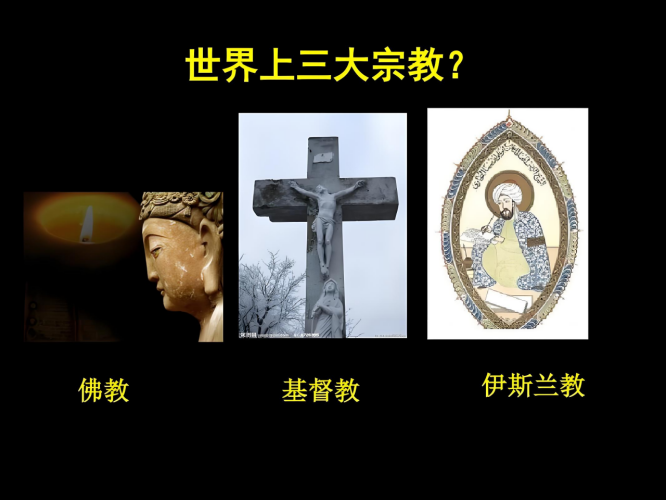
\includegraphics[width=10cm]{picture/1.png}
		\end{figure}
		\par 
	\end{frame} 
	\begin{frame}
		\frametitle{前摇}
		\begin{figure}[H]
			\centering
			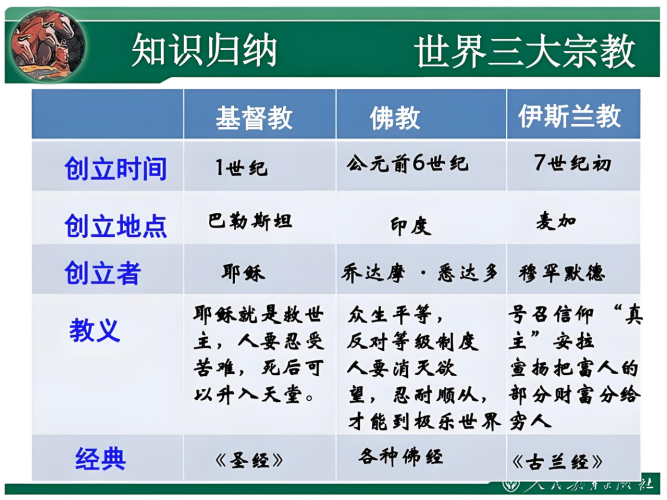
\includegraphics[width=10cm]{picture/2.png}
		\end{figure}
	\end{frame}
	\begin{frame}
		\frametitle{前摇}
		\begin{figure}[H]
			\centering
			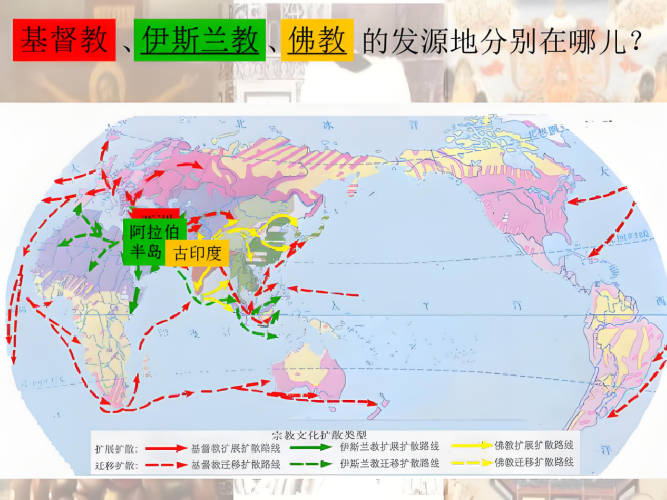
\includegraphics[width=10cm]{picture/3.png}
		\end{figure}
	\end{frame}
	%\chapter{正片}
	\begin{frame}
		\titlepage
	\end{frame}
	\begin{frame}{基督教与天主教的区别}
		很多人将天主教和基督教混为一谈,其实这是不对的。\par\pause
		
		天主教将第一日(星期天)定为“圣日”,但是圣经上明确记载了第七日(星期六)为安息日。\par\pause
		
		【创2:1-3】天和地,以及万象都完成了。到第七日,上帝已经完成了造物之工,就在第七日安息了,歇了他所做一切的工。\textcolor{red}{上帝赐福给第七日,将它分别为圣},因为在这日,上帝安息了,歇了他所做一切创造的工。\par\pause
		
		很明显可以看出天主教是不按照圣经来的。
		
	\end{frame}
	\begin{frame}{圣经}
		\begin{figure}[H]
			\centering
			
\includegraphics[width=10cm]{picture/4.png}
		\end{figure}
	\end{frame}
	\begin{frame}{圣经}
		\textcolor{red}{圣经}(Bibble)来自希腊文的 biblos,意味 “那书”。\par\pause
		下面是圣经的各个章节:
		\begin{figure}[H]
			\centering
			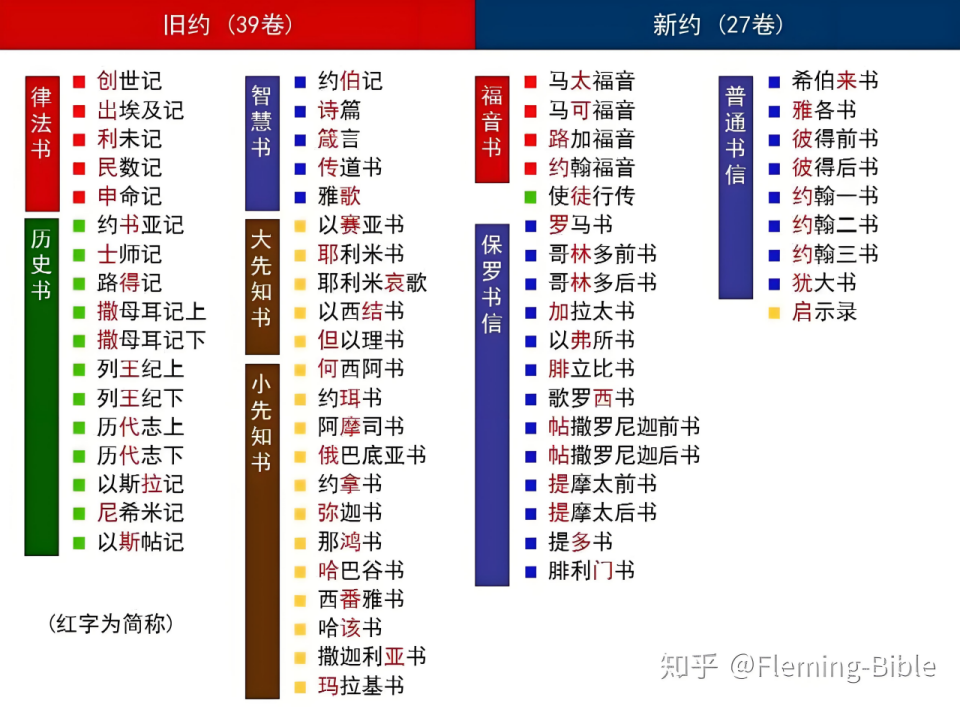
\includegraphics[width=10cm]{picture/5.png}
		\end{figure}
	\end{frame}
	\begin{frame}{圣经}
		由旧约 $39$ 新约 $27$ 卷组成。\par\pause
		圣经是全球\textcolor{red}{印刷量、发行量、销售量、翻译版本最多}的书,曾被带入太空和月球。\par\pause
		圣经有35位左右的记录者。包括有君王和首相,亡国的俘虏和监狱的囚犯,医生、律师、诗人、学者、士官、税吏,渔夫、农人、牧人、工人等。\par\pause
		各个记录者地位不同,环境各异,记录完成于皇宫、监狱、荒岛、旷野及普通民居等。\par\pause
		从旧约圣经开始的公元前1440年,到新约圣经集成的公元397年,时间跨度约1600年。 有个共同的主题:\textcolor{red}{爱}。
	\end{frame}
	\begin{frame}{涉及内容最丰富的一本书}
		圣经共66卷,1189章,30000多节,约935000多字,其中包含历史、诗歌、故事、预言、格言、传记、书信、寓言、比喻、辩论、游记、律法、礼仪、戏剧、哲学、地质、神学、文学、医学、科学、商业、天文、地理、军事、生理、数学、物理、人权、环保、道德律、优生学、心理学、考古学、劳工权益、信息科技、谜语等包罗万有的内容。\par\pause
		来看看其中的一个诗歌:
	\end{frame}
	\begin{frame}{【林前13:4-8】}
		爱的真谛爱是恒久忍耐、又有恩慈。爱是不嫉妒。爱是不自夸。不张狂。\par
		不作害羞的事。不求自己的益处。不轻易发怒。不计算人的恶。\par
		不喜欢不义。只喜欢真理。\par 
		凡事包容。凡事相信。凡事盼望。凡事忍耐。\par 
		爱是永不止息。
	\end{frame}
	\begin{frame}{预言最多的一部书}
		全本圣经有三分之一以上的篇幅是预言。\par \pause
		经统计,旧约预言约 $1239$ 个,新约 $578$ 个,共 $1817$ 个预言。涉及到预言的经文达 $8352$ 句之多。\par \pause
		这里摘录了其中的一个预言。
	\end{frame}
	\begin{frame}{预言}
		【但2:31-35】王啊,你梦见一个大像,这像甚高,极其光耀,站在你面前,形状甚是可怕。\textcolor{red}{这像的头是精金的,胸膛和膀臂是银的,肚腹和腰是铜的,腿是铁的,脚是半铁半泥的}。你观看,见有一块非人手凿出来的石头打在这像半铁半泥的脚上,把脚砸碎;于是金、银、铜、铁、泥都一同砸得粉碎,成如夏天禾场上的糠秕,被风吹散,无处可寻。打碎这像的石头变成一座大山,充满天下。
		\pause
		\begin{wrapfigure}[9]{i}{0cm}
			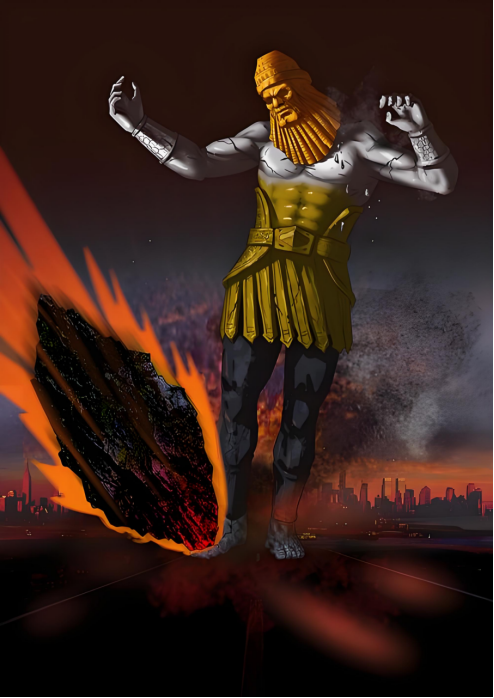
\includegraphics[width=2cm]{picture/6.png}
		\end{wrapfigure}
		\pause
		金头~~~~~~~~~~~~~~~~巴比伦~~~~~~~~强大辉煌\par
		~\par
		\pause
		银胸~~~~~~~~~~~~~~~~玛代-波斯~~~~次之\par
		~\par
		\pause
		铜腰~~~~~~~~~~~~~~~~希腊~~~~~~~~~~~扩张\par
		~\par
		\pause
		铁腿~~~~~~~~~~~~~~~~罗马~~~~~~~~~~~强大持久\par
		~\par
		\pause
		半铁半泥的脚~~~~现在的国家\par 
		~\par
	\end{frame}
	\begin{frame}{关于圣诞节}
		现在的圣诞节是 $12$ 月 $25$ 日,声称是“耶稣诞生的日子”。其实圣经上并没有记载相关日子。\par\pause
		我们可以推理得出“圣诞日”绝对不是在 $12$ 月 $25$ 日。\par\pause
		【路2:12】你们要看见一个婴孩,包着布,卧在马槽里,那就是给你们的记号。\par\pause
		可以看到,耶稣是降生在马槽里的。\pause 用脑子想想都知道,现在的圣诞节是一个大冬天。\par\pause
		由此,圣诞节并不是耶稣降生的日子。只是罗马帝国所敬拜的太阳神的诞辰日。\par\pause
		此外,公元 1 年也不是耶稣降生的日子。\par
	\end{frame}
	\begin{frame}{耶稣被钉的原因}
		\pause
		\begin{itemize}
			\item 直接原因:被钉最后一周骑驴驹进入耶路撒冷圣殿,(当时的敬拜的圣殿成了牛羊卖买的场所),耶稣赶出做买卖的人洁净圣殿。\par\pause
			\item 主要原因:耶稣所传讲天国的福音触犯了统治者的权威,百姓都拥护他,犹太宗教领袖怕被推翻政权,而污告耶稣反叛、并安息日行事的罪,判他钉十字架的罪(罗马最残酷的用刑)。\par\pause
		\end{itemize}
		他为拯救众人而背负罪行接受惩罚,他的圣血洗清人类的罪恶,他的死亡让人们得到救赎。这是基督教的真正教义。
	\end{frame}
	\begin{frame}{}
		谢谢。
	\end{frame}
	
	
	
\end{document}